\chapter{減算型表示を用いた評価実験}
\label{chapter:experiment_dr}
\section{実験の目的}
  看板密集地域において特定の看板を探索する際,加算型の情報提示手法と減算型の情報提示手法を用いたそれぞれの探索時間は,?節で述べたように差がないことが示唆されている.また,減算型情報提示手法には,看板や背景の彩度が低い場合に情報の識別性が加工前との変化が小さくなるという問題点がある.

  そこで本実験では,看板が密集している地域において,加算型情報提示手法と減算型情報提示手法を組み合わせた本稿の提案手法であるハイブリッド型情報提示手法を用いる.この提示手法による探索時間を従来の加算型情報提示手法,減算型情報提示手法と比較することにより,探索時間に関して提案手法の優位性を確認する.



\section{実験の概要}
  実験参加者は情報系の学部に通う大学生12名である.本実験で比較する提示手法は,?節で述べた通常型,加算型,減算型,ハイブリッド型の4種類である.実験は?で述べたプロトタイプをASUS社\footnote{\url{https://www.asus.com/}(2017/4/27確認)}のNexus 7(2013,Android 6.0.1)にインストールして行った.

  実験参加者図は図\ref{fig:exp}に示すように立った状態で端末を持ち,端末を全方向に向けることで全天球画像を見回し,提示された看板を探索する.ユーザが看板を記憶することを防止するために,必ず看板に背を向けた状態で実験を始めるよう指示を出した.実験の条件は,表\ref{tab:order}に示す8通りとした.ここで探索対象の看板数に関して,単体である場合と複数である場合の2通りに区別した.これは探索対象の看板が複数である場合,不要な情報を減算する方が情報を加算することに比べてより容易に情報を探索でき,探索時間が短くなると仮説を立てたためである.

\section{実験の手順}
  初めに,端末の画面が図\ref{fig:experiment} - (a) の状態で実験参加者に端末を渡す.画面には探索対象の看板画像が表示されている.ユーザが開始ボタンをタップすると,図\ref{fig:experiment} - (b) に示す探索画面に遷移する.次に,ユーザが振り返ると,図\ref{fig:experiment} - (c) に示す新日本新地ビルの看板があり,ユーザはその中から探索対象の看板を探す.ユーザが探索対象の看板に1秒間照準を合わせると,図\ref{fig:experiment} - (d) に示す終了画面に遷移する.探索対象が複数である場合は,全ての看板を見つけた後に遷移する.

  実験では,全ての実験参加者に表\ref{tab:order}の条件で探索してもらった.探索対象が単体である条件(表\ref{tab:order},1〜4),探索対象が複数である条件(表\ref{tab:order},5〜8)の順に,昼間の画像と夜の画像でそれぞれ探索してもらった.

  \begin{table}[tb]
    \caption{実験の条件}
    \label{tab:order}
    \begin{center}
    \begin{tabular}{ccc}
      \hline\hline
      \textbf{番号} & \multicolumn{1}{c}{\textbf{提示手法}} & \textbf{対象} \\
      \hline
      1 & 通常型 & 単体 \\
      2 & 加算型 & 単体 \\
      3 & 減算型 & 単体 \\
      4 & ハイブリッド型 & 単体 \\
      \hline
      5 & 通常型 & 複数 \\
      6 & 加算型 & 複数 \\
      7 & 減算型 & 複数 \\
      8 & ハイブリッド型 & 複数 \\
      \hline
    \end{tabular}
  \end{center}
  \end{table}

  \begin{figure}[tb]
    \begin{center}
      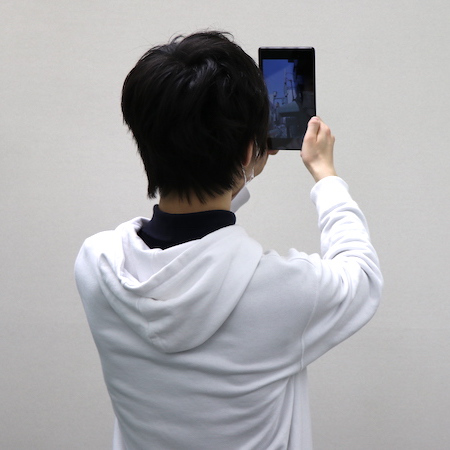
\includegraphics[clip, width=.5\columnwidth]{dr_exp.png}
      \caption{実験風景}
    \end{center}
    \label{fig:exp}
  \end{figure}

  \begin{figure}[t]
    \begin{minipage}{0.49\hsize}
        \begin{center}
            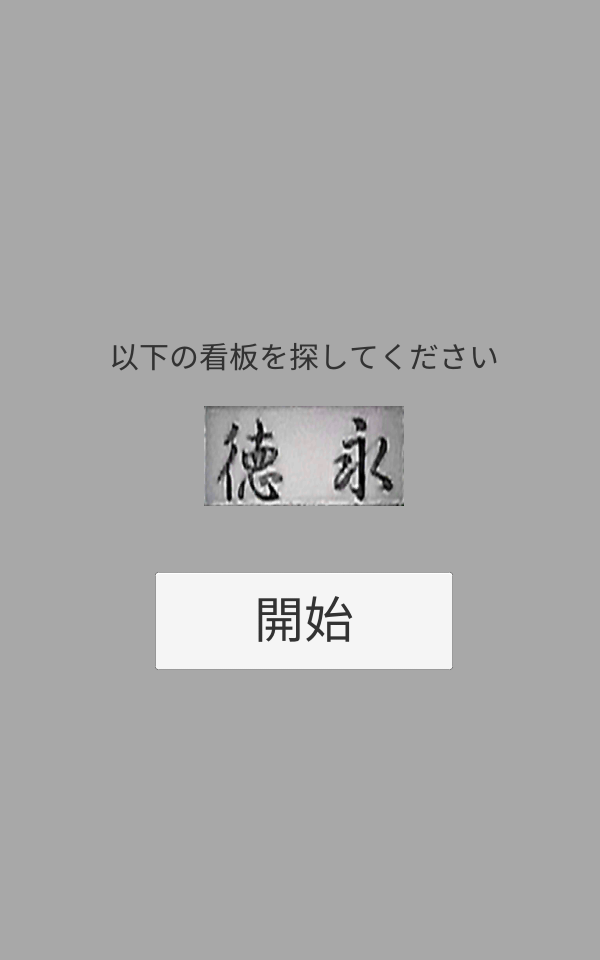
\includegraphics[clip, width=.8\textwidth]{dr_exp1.png}\\
            \small{(a) 開始画面}
        \end{center}
    \end{minipage}
    \begin{minipage}{0.49\hsize}
        \begin{center}
            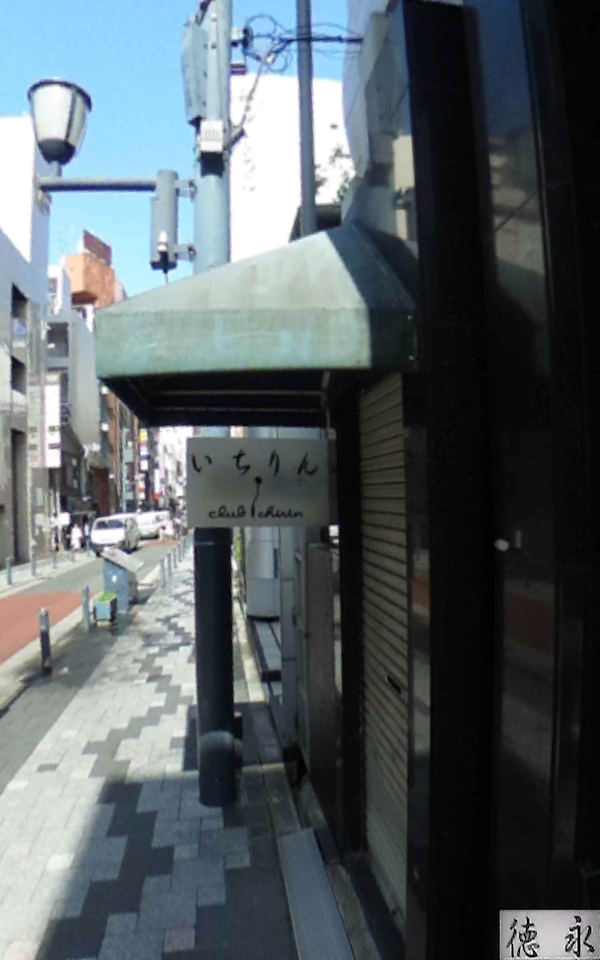
\includegraphics[clip, width=.8\textwidth]{dr_exp2.png}\\
            \small{(b) 探索画面(1)}
        \end{center}
    \end{minipage}
    \begin{minipage}{0.49\hsize}
        \begin{center}
            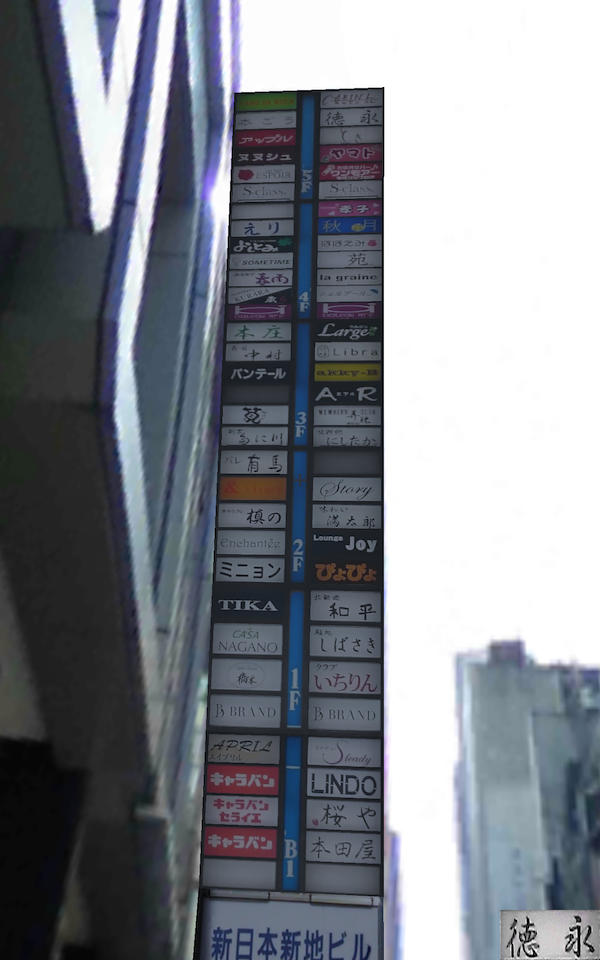
\includegraphics[clip, width=.8\textwidth]{dr_exp3.png}\\
            \small{(c) 探索画面(2)}
        \end{center}
    \end{minipage}
    \begin{minipage}{0.49\hsize}
        \begin{center}
            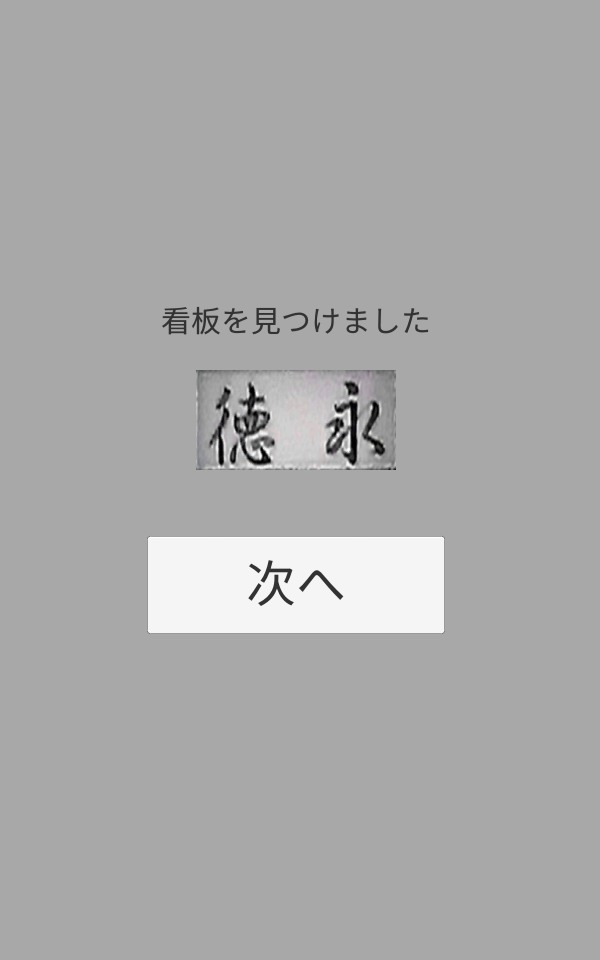
\includegraphics[clip, width=.8\textwidth]{dr_exp4.png}\\
            \small{(d) 終了画面}
        \end{center}
    \end{minipage}
    \vspace{1pt}
    \caption{実験の手順}
    \label{fig:experiment}
  \end{figure}

\section{実験の結果}
  実験参加者が開始ボタンをタップしてから,指示された看板を全て見つけるまでの所要時間を計測し,通常型,加算型,減算型各々の探索時間とハイブリッド型の探索時間の平均値を比較した.その結果を以下に述べる.
  \subsection{時間帯が昼,探索対象が単体の場合}
    時間帯が昼,探索対象が単体の場合の探索時間を図\ref{fig:result1} - (a) に示す.ハイブリッド型を用いた探索時間は,
    (1)通常型より有意に短い($t(22)=5.729,p<.05$)こと,
    (2)加算型より有意に短い($t(22)=2.852,p<.05$)ことが確認されたが,
    (3)減算型との間に有意差は見られなかった($t(22)=1.478,n.s.$).

  \subsection{時間帯が昼,探索対象が複数の場合}
    時間帯が昼,探索対象が複数の場合の探索時間を図\ref{fig:result1} - (b) に示す.ハイブリッド型を用いた探索時間は,
    (1)通常型より有意に短い($t(22)=5.702,p<.05$)こと,
    (2)加算型より有意に短い($t(22)=6.144,p<.05$)こと,
    (3)減算型より有意に短い($t(22)=3.318,p<.05$)ことがそれぞれ確認された.

  \subsection{時間帯が夜,探索対象が単体の場合}
    時間帯が夜,探索対象が単体の場合の探索時間を図\ref{fig:result2} - (a) に示す.ハイブリッド型を用いた探索時間は,
    (1)通常型より有意に短い($t(22)=4.325,p<.05$)こと,
    (2)加算型より有意に短い($t(22)=2.103,p<.05$)こと,
    (3)減算型より有意に短い($t(22)=2.485,p<.05$)ことがそれぞれ確認された.

  \subsection{時間帯が夜,探索対象が複数の場合}
    時間帯が夜,探索対象が複数の場合の探索時間を図\ref{fig:result2} - (b) に示す.ハイブリッド型を用いた探索時間は,
    (1)通常型より有意に短い($t(22)=5.512,p<.05$)こと,
    (2)加算型との間に有意差はない($t(22)=1.857,n.s.$)こと,
    (3)減算型より有意に短い($t(22)=3.129,p<.05$)ことがそれぞれ確認された.

  \subsection{アンケート結果}
    実験終了後に,最も対象の看板を見つけやすかった提示手法についてアンケートを実施したところ,実験参加者の過半数が提案手法であるハイブリッド型情報提示手法を選択した.
  \begin{figure}[t]
      \begin{minipage}{0.49\hsize}
          \begin{center}
              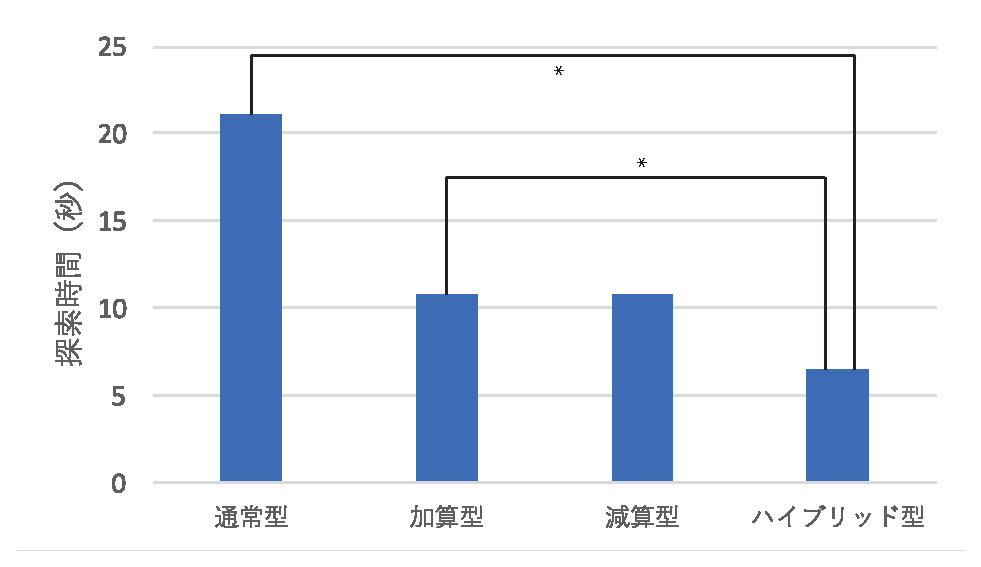
\includegraphics[clip, width=.95\textwidth]{dr_result1.eps}\\
              \small{(a) 対象:単体}
          \end{center}
      \end{minipage}
      \begin{minipage}{0.49\hsize}
          \begin{center}
              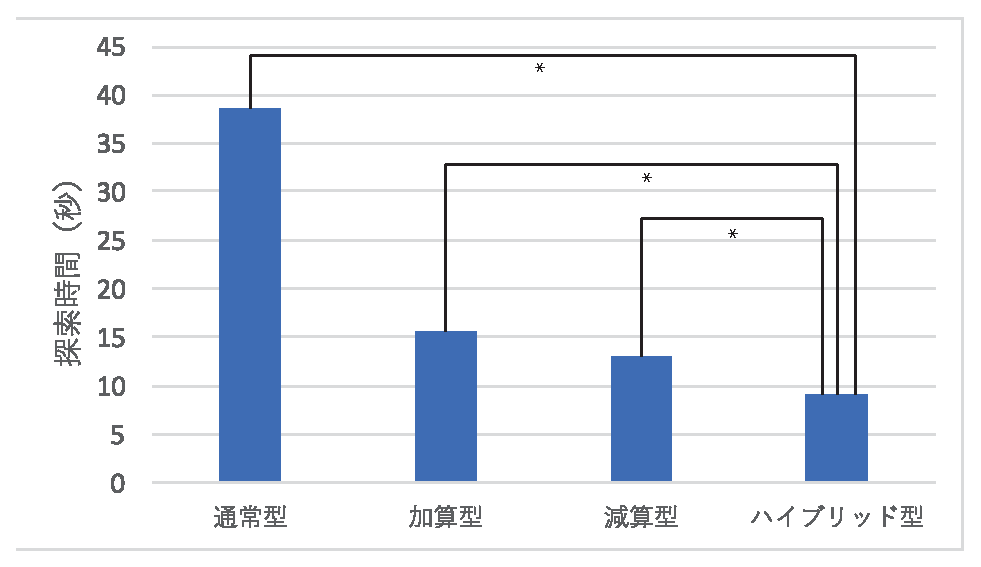
\includegraphics[clip, width=.95\textwidth]{dr_result2.eps}\\
              \small{(b) 対象:複数}
          \end{center}
      \end{minipage}
      \vspace{2pt}
      \caption{実験結果:昼($*:p<.05$)}
      \label{fig:result1}
  \end{figure}
  \begin{figure}[t]
      \begin{minipage}{0.49\hsize}
          \begin{center}
              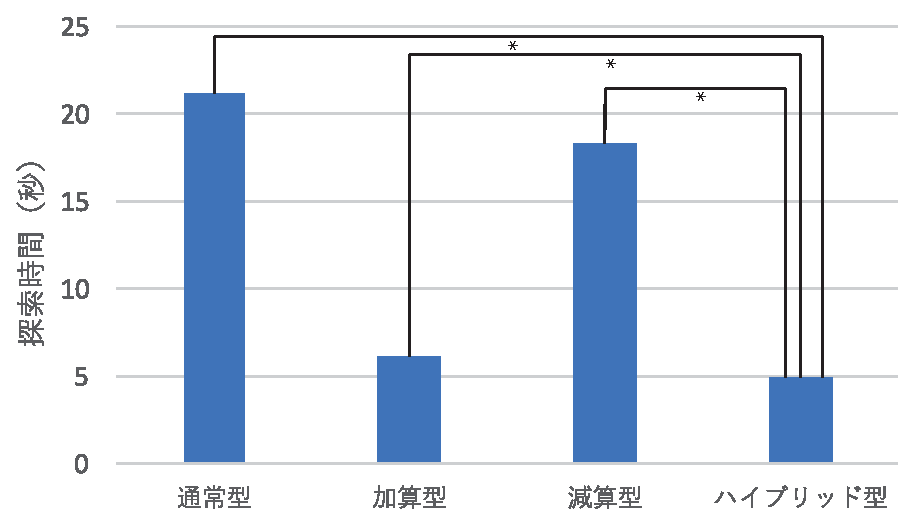
\includegraphics[clip, width=.95\textwidth]{dr_result3.eps}\\
              \small{(a) 対象:単体}
          \end{center}
      \end{minipage}
      \begin{minipage}{0.49\hsize}
          \begin{center}
              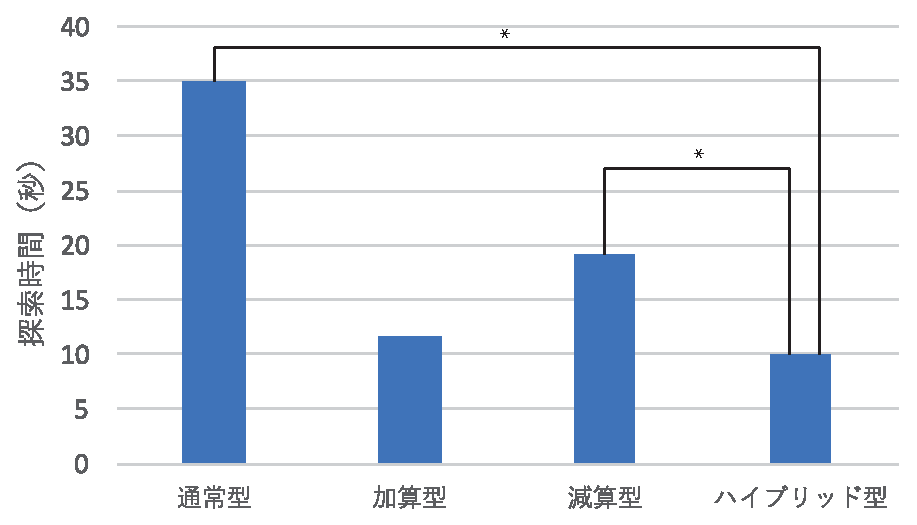
\includegraphics[clip, width=.95\textwidth]{dr_result4.eps}\\
              \small{(b) 対象:複数}
          \end{center}
      \end{minipage}
      \vspace{2pt}
      \caption{実験結果:夜($*:p<.05$)}
      \label{fig:result2}
  \end{figure}

\section{考察}
\label{Consideration}
\subsection{実験結果に関して}
  ?章で述べた実験では,探索対象が単体であり,時間帯が昼の場合,提案手法であるハイブリッド型情報提示手法は文献\cite{Fujita:2013}で提案された減算型情報提示手法と探索時間に関して有意差は見られなかった.しかし,探索対象が複数の場合及び時間帯が夜で探索対象が単体の場合においては,提案手法は減算型情報提示手法よりも探索時間が有意に短いことが確認された.このことから,背景の彩度が低い場合や複数の看板を探索する場合において,提案手法は有効であると考えられる.また,時間帯が夜で探索対象が複数である場合,加算型情報提示手法と比較して減算型情報提示手法の方が探索時間が長くなる傾向が見られた.これは実験に用いた写真の背景の彩度が低かったこと,新日本新地ビルの看板に白と黒から構成されているものが多く含まれていたことにより,減算の効果が減少したことが原因と考えられる.
\subsection{提案インタフェースで達成されたこと}
  本稿では,文献\cite{Fujita:2013}で提案された減算型情報提示手法に文字情報を追加した加算型と減算型のハイブリッド型情報提示手法を提案した.提案手法を用いたシステムのプロトタイプを実装することにより,減算型情報提示手法の問題点であった,不要な情報を減算する際に対象となる看板が白黒であり,かつその周辺の景色の彩度が低い場合に減算の効果が減少するという点が解消されたと考えられる.これにより,彩度が低い環境においても分かりやすい情報提示が可能となった.また,実験結果から看板を探索する際,提案手法を用いることによって探索時間が短くなることが確認された.以上により,?章で述べた看板密集地域における視覚情報の識別性の向上,及び探索時間の短縮が可能になった.
